\section{MediaSense}
MediaSense is a distributed middleware platform for the Internet of Things. It provides a scalable platform with a real time access to context information \cite{Kanter539187}. MediaSense allows support for applications and services to collect and share context information. This, in turn, enables users to focus on developing applications and services without needing to focus on how the context information is shared and how the layers in the platform are interacting with each other \cite{Walters413794}. 

\subsection{Distributed}
MediaSense is using a distributed peer-to-peer overlay to connect all the endpoints in the network. Context information is then persisted and shared in real-time among the nodes in the network. Each node in the network is both a producer and consumer enabling bidirectional access to context information. The overlay used is P-Grid \cite{aberer2003p}. With a lot of users running applications and sharing context information, it is critical that the overlay structure is reliable and scalable \cite{aberer2003p}. P-Grid is self organizing allowing it to scale well. 

\subsection{Applications}
MediaSense is written in the programming language Java and provides an API that can be used to communicate with the platform. The communication from one platform on a device to another device running the platform is done with messages. The API provides methods for registering new context information and find nodes holding specific context information. Each node attached to the network generates information on a continual basis that is accessed and used by other nodes wishing to do so. In order to do this each node register UCIs (Universal Context Identifier). The UCI is stored in the distributed network and other nodes can resolve this and get the address where some required information is stored. When a MediaSense instance gets a message, the dissemination layer of MediaSense handles this message and sends it to the application. The dissemination layer acts like a router delivering messages to the right place. Applications have a method for handling messages that are routed from the dissemination layer. 

\begin{figure}[t]
	\centering
	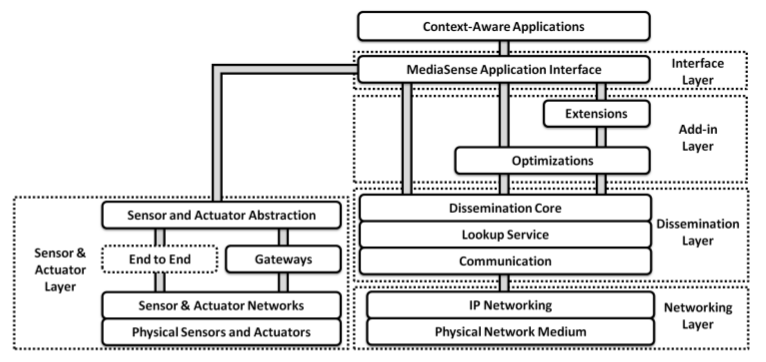
\includegraphics[scale=0.50]{part_2/mediasense/ms_arch.png} 	
	\caption{MediaSense component architecture \cite{Kanter539187} }
\end{figure}

\subsection{Messages}
As mentioned MediaSense communicates with messages. Applications can register what messages they are interested in. When the platform gets a new message from another node in the network, the message will be handled by the dissemination core, which then sends the message to the application on the platform interested in this message. There are several types of messages. The table \ref{tab:table} shows the primitive messages that are available for registering and retrieving information. 

\begin{center}
\begin{table}
    \begin{tabularx}{\textwidth}{ | l | X |}
    \hline
    Message name 		& 		Description \\ \hline
	REGISTER UCI 		& 		Registers a UCI along with the node which is responsible for it. \\ \hline
	RESOLVE UCI 		& 		Resolves a UCI to the node which is responsible for it. \\ \hline
	GET 				& 		Fetches the current context value from the node responsible for a UCI. The reply is sent using a NOTIFY. \\ \hline
	SET 				& 		Changes the current status of an actuator in an end point. \\ \hline
	SUBSCRIBE 			& 		Makes a subscription request to the node responsible for a UCI, The node then sends a NOTIFY message containing the current context value, either at regular intervals or when the value changes. \\ \hline
	NOTIFY 				& 		Notifies an interested node of the current context value associated with a specified UCI. \\ \hline
	TRANSFER 			& 		Requests the manager of a resource to transfer responsibility to another node. This might be full or partial responsibility, where the requester re-creates a copy of the resource permitting improved real time performance. \\ \hline
    \end{tabularx}
	\caption{Primitive messages in MediaSense}
	\label{tab:table}
\end{table}
\end{center}


\subsection{MediaSense Execution}
When an application wishes to use the MediaSense platform, the application must initialize and use its own instance of MediaSense. Therefore, a user running two applications at the same time must initialize two instances of the platform. Every instance of MediaSense is seen as a separate node, so if we have two instances of the platform on one device this device is acting as two nodes in the network. This is misleading because one node in the network should be one device and not one application.

\begin{figure}[t]
	\centering
    	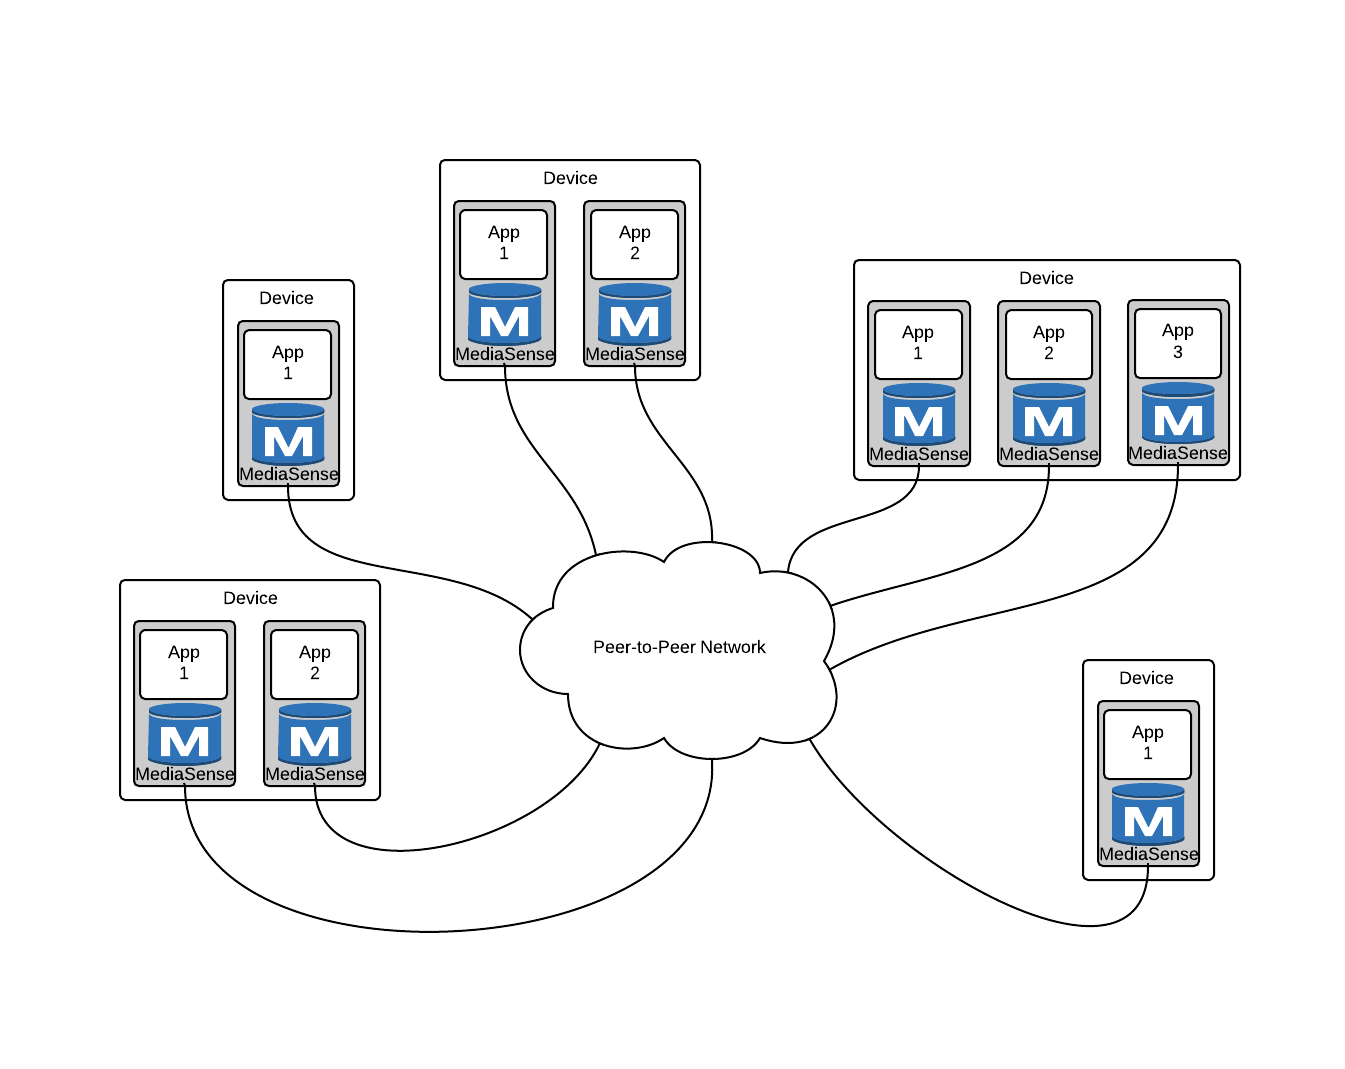
\includegraphics[scale=0.25]{part_2/mediasense/several_nodes_on_one_device.png}
		\caption{Figure showing how the instances of MediaSense is connected to the network} 
\end{figure}

Each instance of MediaSense requires that a new port be opened so the network layer can communicate with other nodes in the network. This means that if the user is behind a NAT or a firewall the user needs to open up new ports for every instance of MediaSense. The amount of open ports is equal to the amount of applications running on a device. This is a security issue. With more ports opened, the device that is running the platform is more vulnerable to different kinds of attacks. Not only that the device will be more vulnerable, when a user needs several instances of MediaSense and every instance need its own port the network usage will increase. This can affect the battery time of low resource devices in a negative way.

One more thing to consider with an application invoked platform is that the memory usage will increase. Every instance of MediaSense needs to use a specific amount of memory. If the platform is running on a resource constrained device, this will limit the number of applications running on the device, because of the several instances of MediaSense. This is contradictory to the requirement defined by Kanter et al. \cite{Kanter539187} that Internet of Things Middleware should be lightweight.

To make MediaSense more efficient, we need to reduce the resource footprint without losing  the functionality. This can be done in several ways. One way is to change the overlay architecture and use a centralized approach for sharing and collecting context information. This solution will make every application connect to a centralized server or to use an internet portal, for example, RESTful API, to access the data. The problem with this solution is that it is centralized and, therefore, does not scale well. Additionally, the functionality of P-Grid will be lost. They are also dependent on DNS which means that applications expect that the centralized server always is available. As mentioned previously, centralized solutions are more vulnerable and can be attacked with Denial-of-service attacks. If the centralized server is having DNS errors the context information can not be accessed or shared to other applications, and the applications become unusable. Examples of Internet of thing services using this architecture are SenseWeb and Sensei. These two examples use centralized web-services for sharing context information, which makes them have the mentioned reliability issues and are consequently not a good solution for an Internet of things service.

\begin{center}
\begin{table}
    \begin{tabularx}{\textwidth}{ |X|X|X|X| }
    \hline
    Number Of Applications 								& Memory Usage 									& CPU Time							& Threads\\ \hline
    1 													& 70.4 MB 										& 2.70 								& 30 \\ \hline
    2 													& 139.2 MB										& 5.34 								& 60 \\ \hline
    3 													& 213.04 MB										& 8.72 								& 90 \\ \hline
    4 													& 286.5 MB										& 12.88 							& 120 \\ \hline
    5													& 360.2 MB										& 15.43  							& 150 \\ \hline
    6													& 430.3 MB										& 18.82  							& 180 \\ \hline	
    7													& 505.3 MB										& 21.54  							& 210 \\ \hline
    8													& 574.1 MB										& 24.85  							& 240 \\ \hline
    9													& 648.3 MB										& 27.84	  							& 270 \\ \hline
    10													& 718.3 MB										& 31.25  							& 300 \\ \hline
    \end{tabularx}
   	\caption{This table shows how much resource is in use when MediaSense is running}
	\label{tab:test_table}
\end{table}
\end{center}
